\subsection{Multilayer Perceptron}

\begin{frame}[fragile]
\frametitle{Multilayer Perceptron}

\hspace{-5mm}

\begin{itemize}
\item In Grundzügen bereits beim Backpropagation Algorithmus erläutert 
\end{itemize}

\hspace{5mm}

\begin{columns}

\begin{column}{.5\textwidth}
\begin{figure}
	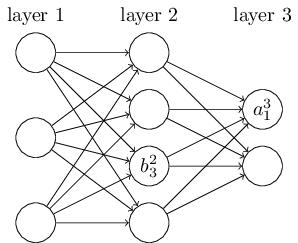
\includegraphics[width=\linewidth]{./zusatz/multilayerPerceptron/img/biasAct_notation}
\end{figure}
\end{column}

\begin{column}{.5\textwidth}

Anwendungsbereiche: 
\begin{itemize}
\item Mustererkennung 
\item Funktionenapproximation
\item Klassifizierung
\item Prognose
\item Diagnose
\item Steuerung 
\item Optimierung
\end{itemize}
\end{column}

\end{columns}

\note[item]{vielfältige Struktur}
\note[item]{Mehrschichtiges Netz, bereits beim BPAlgo. verwendet}
\note[item]{Zu tiefe Netz: Probleme beim Training}
\note[item]{Techniken unter Deep learning zusammengefasst}
\note[item]{Stuktur: mehrschichtiges forwärtsgekoppeltes Netz}
\note[item]{Feedforward: durchiterieren von Eingabewerten}
\note[item]{}
\note[item]{}

\end{frame}



\begin{frame}[fragile]
\frametitle{Sigmoid Aktivierungsfunktion}

\begin{columns}

\begin{column}{.5\textwidth}
\begin{itemize}
\item Einfach / schnell zu berechnen
\item Einfach / schnell abzuleiten
\end{itemize}
\end{column}

\begin{column}{.5\textwidth}
\myeq{
f(x) & = \frac{1}{1 + exp(-b * x)} \\
f'(x) & = b * f(x)(1-f(x))
}
\end{column}

\end{columns}

\begin{figure}
	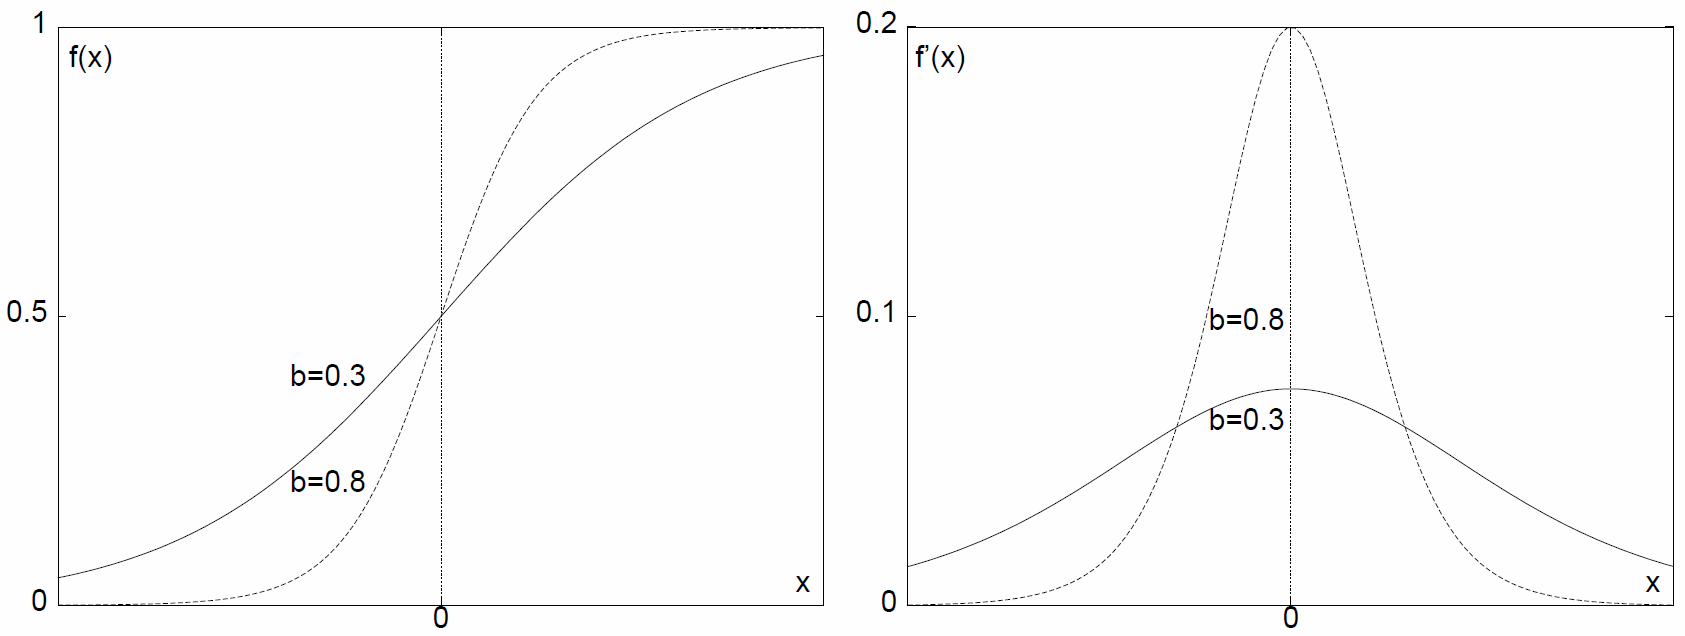
\includegraphics[width=\linewidth]{./zusatz/multilayerPerceptron/img/plotSigmoid_alpha}
\end{figure}

\note[item]{Wertebereich: zwischen 0 und 1}
\note[item]{Konstante berschreibt Steilheit der Kurve}
\note[item]{Über die komplette Domäne differenzierbar}

\end{frame}
